\documentclass[letterpaper,12pt,fleqn]{article}
\usepackage{matharticle}
\usepackage{mathtools}
\usepackage{tikz}
\pagestyle{plain}
\begin{document}

\begin{center}
\Large Math-08 Homework \#1 Solutions
\end{center}

\vspace{0.5in}

\underline{Reading}

\begin{itemize}
\item If necessary, skim through the documents in the resources module on
  canvas dealing with mathematical logic, sets, rational numbers, and prime
  factorization. The documents have more information than you will need;
  however, if you have something in your notes that you do not understand then
  you can find more description in the documents.
\item Text book sections 0.1 and 0.2.
\end{itemize}

\underline{Problems}

\begin{enumerate}
\item Let:
\begin{eqnarray*}
P &\coloneqq& 0\ \mbox{is a positive number} \\
Q &\coloneqq& 0\ \mbox{is a rational number} \\
\end{eqnarray*}
Determine whether the following are true or false:
\begin{enumerate}
\item P
  
  $0$ is neither positive nor negative, so the statement is FALSE.
  
\item Q

  $0$ can be written as $\frac{0}{1}$, a ratio of two integers where the
  denominator is not $0$. Thus, the statement is TRUE.
  
\item not P

  not FALSE = TRUE
  
\item not Q

  not TRUE = FALSE
  
\item P and Q

  For an AND statement to be true, both statements must be true. Since P is
  false, the statement is FALSE:

  FALSE and TRUE = FALSE

\item P or Q

  For an OR statement to be true, at least one of the statements must be true.
  Since Q is true, the statement is TRUE:

  FALSE or TRUE = TRUE
  
\end{enumerate}
\newpage
\item Decimal to rational form conversion.
\begin{enumerate}
\item Convert $0.14\overline{23}$ to rational form.

  Let $x=0.14\overline{23}$

  Multiply $x$ by $100$ to capture all of the non-repeating digits to the left
  of the decimal point:

  $100x=14.\overline{23}$

  Now multiply $x$ by $10000$ to capture the non-repeating digits and one set
  of the repeating digits to the left of the decimal point:
  
  $10000x=1423.\overline{23}$

  Now subtract so that the repeating digits on the right of the decimal point
  cancel and then solve for $x$:

  \begin{eqnarray*}
    10000x-100x &=& 1423.\overline{23} - 14.\overline{23} \\
    9900x &=& 1409 \\
    x &=& \frac{1409}{9900} \\
  \end{eqnarray*}

\item Show that $0.\overline{1} = \frac{1}{9}$.

  \begin{eqnarray*}
    x &=& 0.\overline{1} \\
    10x &=& 1.\overline{1} \\
    10x-x &=& 1.\overline{1}-0.\overline{1} \\
    9x &=& 1 \\
    x &=& \frac{1}{9} \\
  \end{eqnarray*}
  
\item If this is so, then $\frac{2}{9}$ should equal $0.\overline{2}$,
  $\frac{3}{9}$ should equal $0.\overline{3}$, and so on until $\frac{8}{9}$
  should equal $0.\overline{8}$. So, what do you think that $0.\overline{9}$
  should equal?

  According to the pattern, $0.\overline{9}$ should equal $\frac{9}{9}$, which
  equals $1$. This demonstrates the fact that when an infinite decimal value is
  arbitrarity close to an exact value, then the two values are considered to be
  equal.
\newpage
\item Show that this is so by converting $0.\overline{9}$ to rational form.

  \begin{eqnarray*}
    x &=& 0.\overline{9} \\
    10x &=& 9.\overline{9} \\
    10x-x &=& 9.\overline{9}-0.\overline{9} \\
    9x &=& 9 \\
    x &=& \frac{9}{9} \\
    x &=& 1 \\
  \end{eqnarray*}
  
\item Take a guess at what $25.3\overline{9}$ equals.

  Note that this value gets arbitrarily close to $25.4$.
\end{enumerate}

\item Rational numbers and closure.
  \begin{enumerate}
  \item Write down the definition of $\Q$ using setbuilder notation.

    \[\Q=\left\{\frac{p}{q}\mid p,q\in\Z\ \mbox{and}\ q\ne0\right\}\]
    
  \item Prove that $\Q$ is closed under addition (Hint: Assume that two numbers
    are in $\Q$, use the definition to express them as a ratio of integers,
    then add then and show why the result must be rational).

    Assume $a,b\in\Q$ \\
    Per the definition, let $a=\frac{p}{q}$ where $p,q\in\Z$ and $q\ne0$ \\
    Also, per the definition, let $b=\frac{r}{s}$ where $r,s\in\Z$ and
    $s\ne0$
    \[a+b=\frac{p}{q}+\frac{r}{s}=\frac{ps+rq}{qs}\]
    Now remember that the integers are closed under addition and multiplication
    (integers make integers), so: \\
    \[ps+rq\in\Z\ \mbox{and}\ qs\in\Z\]
    Furthermore, $q\ne0$ and $s\ne0$, so $qs\ne0$
    
    Thus, the result meets the definition of a rational number. Since our
    choice of $a$ and $b$ was arbitrary, this result holds for any two
    rational numbers.  Therefore, $\Q$ is closed under addition.
    \newpage
  \item Prove that $\Q$ is closed under multiplication (Hint: same as above,
    but multiply the two numbers).

    \[a+b=\frac{p}{q}\cdot\frac{r}{s}=\frac{pr}{qs}\]
    \[pr\in\Z\ \mbox{and}\ qs\in\Z\]
    Furthermore, $q\ne0$ and $s\ne0$, so $qs\ne0$

    Thus, the result meets the definition of a rational number. Therefore, $\Q$
    is closed under multiplication.

  \item Give a counterexample showing that $\R-\Q$ is not closed under addition.

    The statement that we wish to test is:
    \[\forall\,a,b\in\R-\Q,a+b\in\R-\Q\]
    Consider the following:
    \[\pi+(-\pi)=0\]
    Both $pi$ and $-pi$ are irrational, but adding them results in $0$, a
    rational number.  This is a counterexample to the statement that the
    irrationals are closed under addition. Therefore, the irrationals are not
    closed under addition.
    
  \item Give a counterexample showing that $\R-\Q$ is not closed under
    multiplication.

    The statement that we wish to test is:
    \[\forall\,a,b\in\R-\Q,ab\in\R-\Q\]
    Consider the following:
    \[\pi\left(\frac{1}{\pi}\right)=1\]

    Both $\pi$ and $\frac{1}{\pi}$ are irrational, but multiplying them results
    in $1$, a rational number.  This is a counterexample to the statement that
    the irrationals are closed under multiplication. Therefore, the irrationals
    are not closed under multiplication.
  \end{enumerate}
\newpage
\item Let:
\begin{eqnarray*}
A &=& \mbox{the set of all positive real numbers} \\
B &=& \mbox{the set of real numbers between -3 (exclusive) and 3 (inclusive)} \\
\end{eqnarray*}
\begin{enumerate}
\item Graph each set on the real number line.

  \bigskip
  
  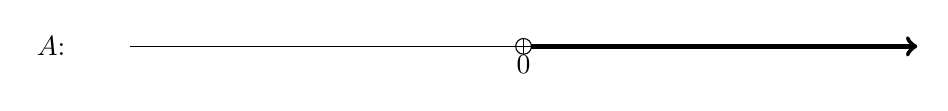
\begin{tikzpicture}
    \node at (-6,0) {$A$:};
    \draw (-5,0) -- (5,0);
    \draw (0,0.1) -- (0,-0.1);
    \node [below] at (0,0) {$0$};
    \draw (0,0) circle [radius=0.1];
    \draw [->,ultra thick] (0.1,0) -- (5,0);
  \end{tikzpicture}
  
  \bigskip
  
  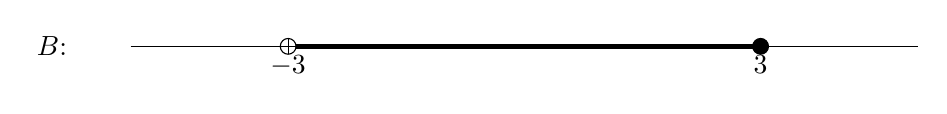
\begin{tikzpicture}
    \node at (-6,0) {$B$:};
    \draw (-5,0) -- (5,0);
    \draw (-3,0.1) -- (-3,-0.1);
    \draw (3,0.1) -- (3,-0.1);
    \node [below] at (-3,0) {$-3$};
    \node [below] at (3,0) {$3$};
    \draw (-3,0) circle [radius=0.1];
    \draw [fill=black] (3,0) circle [radius=0.1];
    \draw [ultra thick] (-2.9,0) -- (2.9,0);
  \end{tikzpicture}
  
\item Represent each set using set-builder notation.
  \[A=\{x\in\R,x>0\}\]
  \[B=\{x\in\R,-3<x\le3\}\]
  
\item Represent each set using interval notation.
  \[A=(0,\infty)\]
  \[B=(-3,3]\]
    
\item Graph $A\cup B$ and represent it in interval notation.

  For an element to be in the union of $A$ and $B$ it must be in $A$ or in
  $B$ (it can be in both!):
  \[A\cup B=\{x\in\R\mid x\in A\ \mbox{or}\ x\in B\}\]
  It helps to draw each graph on top of each other, draw dotted lines through
  all the endpoints, and then determine which regions are included:
    
  \bigskip

  \begin{tikzpicture}
    \node at (-6,4) {$A$:};
    \draw (-5,4) -- (5,4);
    \draw (0,4.1) -- (0,3.9);
    \node [below] at (0,4) {$0$};
    \draw (0,4) circle [radius=0.1];
    \draw [->,ultra thick] (0.1,4) -- (5,4);

    \node at (-6,2) {$B$:};
    \draw (-5,2) -- (5,2);
    \draw (-3,2.1) -- (-3,1.9);
    \draw (3,2.1) -- (3,1.9);
    \node [below] at (-3,2) {$-3$};
    \node [below] at (3,2) {$3$};
    \draw (-3,2) circle [radius=0.1];
    \draw [fill=black] (3,2) circle [radius=0.1];
    \draw [ultra thick] (-2.9,2) -- (2.9,2);

    \node at (-6,0) {$A\cup B$:};
    \draw (-5,0) -- (5,0);
    \draw (-3,0.1) -- (-3,-0.1);
    \node [below] at (-3,0) {$-3$};
    \draw (-3,0) circle [radius=0.1];
    \draw [->,ultra thick] (-2.9,0) -- (5,0);
    \node at (6,0) {$(-3,\infty)$};

    \draw [dashed] (-3,5) -- (-3,-1);
    \draw [dashed] (0,5) -- (0,-1);
    \draw [dashed] (3,5) -- (3,-1);
  \end{tikzpicture}
\newpage
\item Graph $A\cap B$ and represent it in interval notation.

  For an element to be in the intersection of $A$ and $B$ it must be in both
  $A$ and $B$:
  \[A\cap B=\{x\in\R\mid x\in A\ \mbox{and}\ x\in B\}\]
    
  \bigskip

  \begin{tikzpicture}
    \node at (-6,4) {$A$:};
    \draw (-5,4) -- (5,4);
    \draw (0,4.1) -- (0,3.9);
    \node [below] at (0,4) {$0$};
    \draw (0,4) circle [radius=0.1];
    \draw [->,ultra thick] (0.1,4) -- (5,4);

    \node at (-6,2) {$B$:};
    \draw (-5,2) -- (5,2);
    \draw (-3,2.1) -- (-3,1.9);
    \draw (3,2.1) -- (3,1.9);
    \node [below] at (-3,2) {$-3$};
    \node [below] at (3,2) {$3$};
    \draw (-3,2) circle [radius=0.1];
    \draw [fill=black] (3,2) circle [radius=0.1];
    \draw [ultra thick] (-2.9,2) -- (2.9,2);

    \node at (-6,0) {$A\cup B$:};
    \draw (-5,0) -- (5,0);
    \draw (0,0.1) -- (0,-0.1);
    \draw (3,0.1) -- (3,-0.1);
    \node [below] at (0,0) {$0$};
    \node [below] at (3,0) {$3$};
    \draw (0,0) circle [radius=0.1];
    \draw [fill=black] (3,0) circle [radius=0.1];
    \draw [ultra thick] (0.1,0) -- (2.9,0);
    \node at (6,0) {$(0,3]$};

    \draw [dashed] (-3,5) -- (-3,-1);
    \draw [dashed] (0,5) -- (0,-1);
    \draw [dashed] (3,5) -- (3,-1);
  \end{tikzpicture}

  Note that the endpoint $0$ is not included because even though it is in $B$,
  it is not in $A$. On the other hand, the endpoint $3$ is included because it
  is in both $A$ and $B$.
\end{enumerate}
\end{enumerate}
\end{document}
